% !TEX program = xelatex
% Especificacion de Casos de Uso -- Sistema de Inventario + POS (Peterby's)
% Compilar: latexmk -xelatex -output-directory=../_build casos-de-uso.tex
\documentclass[11pt]{article}

\usepackage{fontspec}
\setmainfont{Latin Modern Roman}
\setsansfont{Latin Modern Sans}
\setmonofont{Latin Modern Mono}[Scale=0.92]
\usepackage[spanish,es-tabla,es-nodecimaldot]{babel}
\usepackage{microtype}
\usepackage[a4paper,margin=2.3cm,headheight=22pt]{geometry}
\usepackage{xcolor}
\usepackage{booktabs}
\usepackage{array}
\usepackage{longtable}
\usepackage{graphicx}
\usepackage{enumitem}
\usepackage{titlesec}
\usepackage{fancyhdr}
\usepackage{caption}
\usepackage[most]{tcolorbox}
\usepackage{hyperref}
\usepackage[strings]{underscore} % despues de pgf/tcolorbox y hyperref

\definecolor{brand}{HTML}{34508A}
\definecolor{brandlight}{HTML}{EAF0FA}
\definecolor{rule}{HTML}{C5CEE0}

\hypersetup{colorlinks=true, linkcolor=brand, urlcolor=brand,
  pdftitle={Especificacion de Casos de Uso -- Sistema de Inventario Peterby's},
  pdfauthor={Equipo de Ingenieria de Software}}
\captionsetup{font=small, labelfont={bf,color=brand}}

% --- Encabezado / pie ---
\pagestyle{fancy}
\fancyhf{}
\renewcommand{\headrulewidth}{0.6pt}
\renewcommand{\headrule}{\hbox to\headwidth{\color{rule}\leaders\hrule height \headrulewidth\hfill}}
\fancyhead[L]{\small\sffamily\color{brand}Especificación de Casos de Uso}
\fancyhead[R]{\small\sffamily Peterby's POS}
\fancyfoot[C]{\small\sffamily\thepage}

% --- Titulos ---
\titleformat{\section}{\Large\sffamily\bfseries\color{brand}}{\thesection.}{0.5em}{}
\titleformat{\subsection}{\large\sffamily\bfseries\color{brand!85!black}}{\thesubsection}{0.6em}{}
\titlespacing*{\subsection}{0pt}{1.4ex plus 1ex}{0.6ex}

% --- Ficha de caso de uso ---
\newtcolorbox{ficha}[2]{%
  breakable, enhanced, colback=white, colframe=brand, boxrule=0.7pt,
  coltitle=white, fonttitle=\sffamily\bfseries,
  title={#1\hspace{1.2em}#2},
  left=2.6mm, right=2.6mm, top=1.8mm, bottom=2.2mm,
  before skip=2.6mm, after skip=2.6mm, parbox=false}

% Campo de una sola linea con sangria francesa
\newcommand{\fila}[2]{\par\smallskip\noindent\hangindent=2.8em\hangafter=0
  \textbf{\sffamily\color{brand!80!black}#1.}\hspace{0.4em}#2\par}
% Subtitulo dentro de la ficha
\newcommand{\bloque}[1]{\par\smallskip\noindent\textbf{\sffamily\color{brand!80!black}#1}\par\nopagebreak}

\newlist{pasos}{enumerate}{1}
\setlist[pasos]{label=\arabic*., leftmargin=2.2em, itemsep=0.15ex, topsep=0.3ex}
\newenvironment{alternos}{\begin{itemize}[leftmargin=2.9em, itemsep=0.2ex, topsep=0.3ex]}{\end{itemize}}

\begin{document}

% ===================== PORTADA =====================
\begin{titlepage}
\centering
\vspace*{1.2cm}
{\sffamily\large Instituto Politécnico Nacional}\\[0.2cm]
{\sffamily Escuela Superior de Cómputo --- ESCOM}\\[0.2cm]
{\sffamily Ingeniería de Software}\\[2.2cm]

{\color{rule}\rule{\linewidth}{0.8pt}}\\[0.6cm]
{\Huge\sffamily\bfseries\color{brand} Especificación de Casos de Uso}\\[0.5cm]
{\large\sffamily Sistema de Inventario con Punto de Venta\\ y Análisis Predictivo de Reabastecimiento}\\[0.3cm]
{\large\sffamily\itshape Tienda de ropa Peterby's}\\[0.4cm]
{\color{rule}\rule{\linewidth}{0.8pt}}\\[1.6cm]

\begin{tabular}{rl}
\sffamily\bfseries Actores: & \sffamily Gerente, Vendedor, Sistema \\[0.2cm]
\sffamily\bfseries Casos de uso: & \sffamily 16 \\[0.2cm]
\sffamily\bfseries Documento: & \sffamily Análisis de requerimientos \\
\end{tabular}

\vfill
{\sffamily\small Diciembre 2025}
\end{titlepage}

\tableofcontents
\clearpage

% ===================== 1. INTRODUCCION =====================
\section{Introducción}
Este documento especifica los casos de uso del sistema de inventario y punto de
venta (POS) de la tienda Peterby's. Los casos de uso se derivan de los
requerimientos funcionales (RF), las reglas de negocio (RN) y los actores
identificados en el análisis del sistema. Cada caso de uso se describe con una
ficha que incluye actores, objetivo, precondiciones, flujo principal, flujos
alternos, postcondiciones y las reglas y requerimientos asociados.

\subsection{Actores}
\begin{description}[leftmargin=0pt, style=nextline, itemsep=0.4ex]
  \item[\sffamily\color{brand!80!black} Gerente] Administra el sistema: catálogos,
    productos, proveedores, promociones, inventario y usuarios; consulta el
    dashboard y los reportes, y atiende las recomendaciones del módulo predictivo.
  \item[\sffamily\color{brand!80!black} Vendedor] Opera el punto de venta:
    registra ventas, procesa devoluciones, consulta existencias y registra
    clientes.
  \item[\sffamily\color{brand!80!black} Sistema (módulo predictivo)] Actor
    secundario que ejecuta procesos automáticos: genera alertas de stock y
    predicciones de reabastecimiento al iniciar el sistema y tras cada venta.
\end{description}

\subsection{Diagramas de casos de uso}
La Figura~\ref{fig:cu-general} presenta la visión general; las
Figuras~\ref{fig:cu-admin} a~\ref{fig:cu-pred} detallan cada módulo con sus
relaciones \texttt{<<include>>} y \texttt{<<extend>>}.

\begin{figure}[htbp]
  \centering
  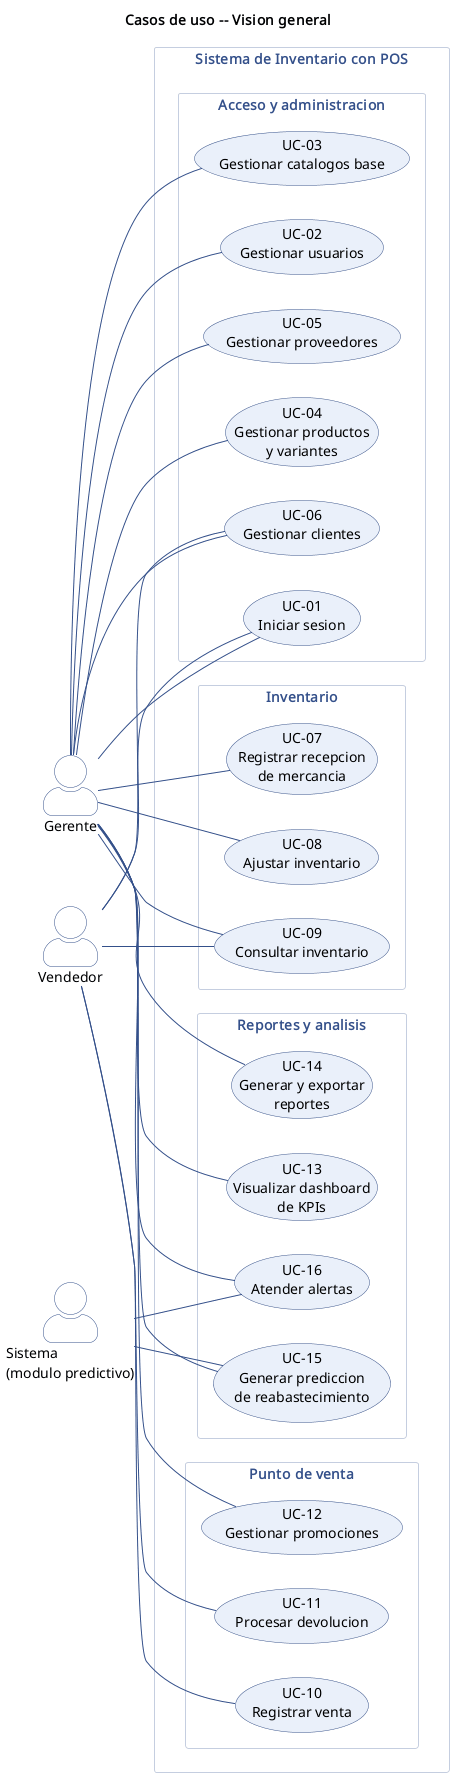
\includegraphics[width=\linewidth,height=0.84\textheight,keepaspectratio]{diagramas/cu-general.png}
  \caption{Diagrama general de casos de uso.}
  \label{fig:cu-general}
\end{figure}

\begin{figure}[htbp]
  \centering
  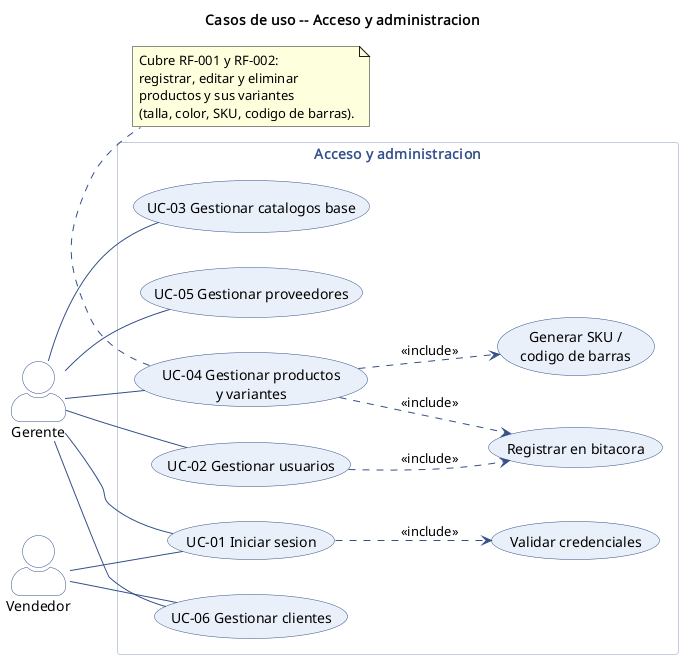
\includegraphics[width=\linewidth,height=0.42\textheight,keepaspectratio]{diagramas/cu-administracion.png}
  \caption{Módulo de acceso y administración.}
  \label{fig:cu-admin}
\end{figure}

\begin{figure}[htbp]
  \centering
  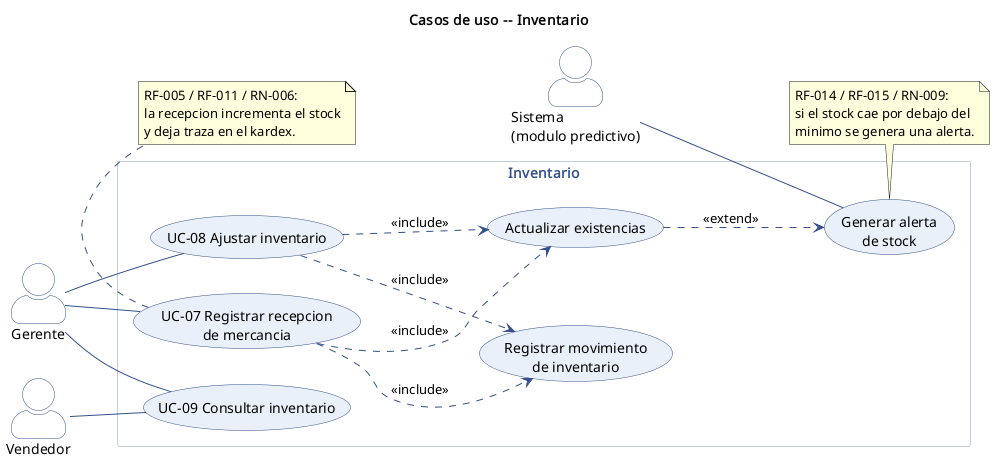
\includegraphics[width=\linewidth,height=0.42\textheight,keepaspectratio]{diagramas/cu-inventario.png}
  \caption{Módulo de inventario.}
  \label{fig:cu-inv}
\end{figure}

\begin{figure}[htbp]
  \centering
  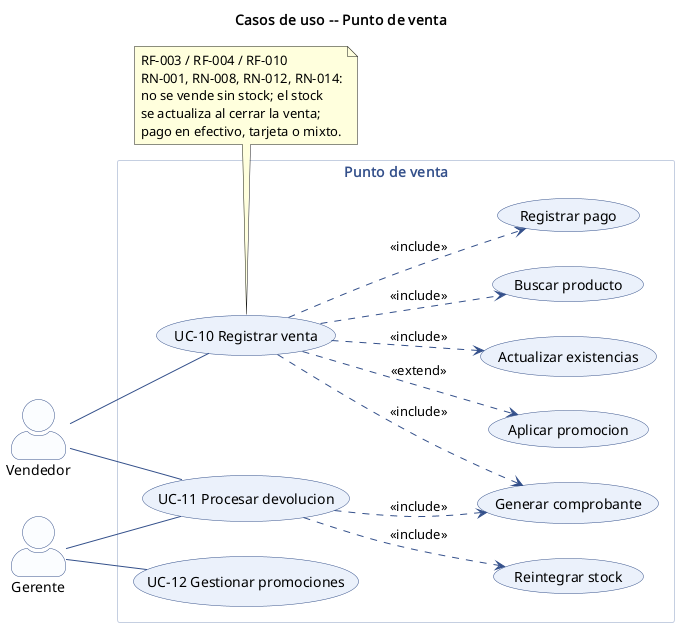
\includegraphics[width=\linewidth,height=0.50\textheight,keepaspectratio]{diagramas/cu-punto-de-venta.png}
  \caption{Módulo de punto de venta.}
  \label{fig:cu-pos}
\end{figure}

\begin{figure}[htbp]
  \centering
  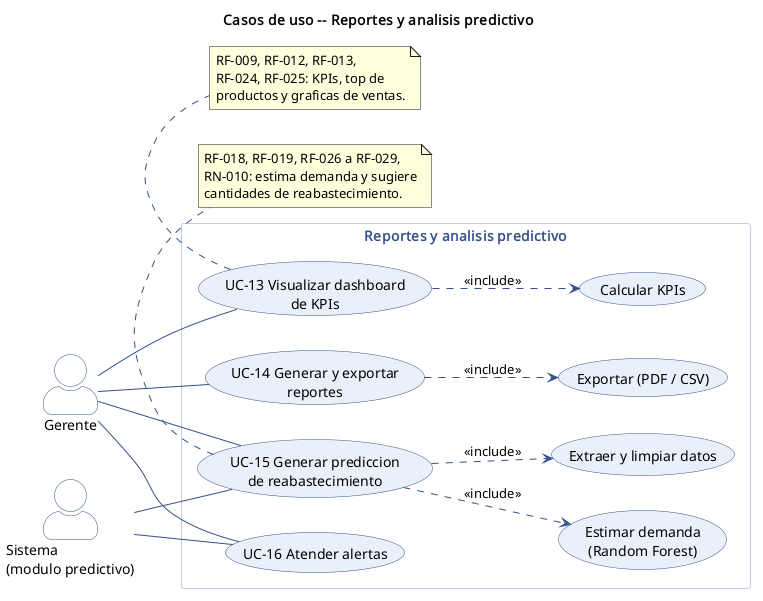
\includegraphics[width=\linewidth,height=0.50\textheight,keepaspectratio]{diagramas/cu-reportes-prediccion.png}
  \caption{Módulo de reportes y análisis predictivo.}
  \label{fig:cu-pred}
\end{figure}
\clearpage

% ===================== 2. CASOS DE USO =====================
\section{Especificación de los casos de uso}

\subsection{UC-01 Iniciar sesión}
\begin{ficha}{UC-01}{Iniciar sesión}
\fila{Actores}{Gerente, Vendedor}
\fila{Objetivo}{Autenticar al usuario y cargar la ventana principal según su rol.}
\fila{Precondiciones}{El usuario tiene una cuenta activa en el sistema.}
\bloque{Flujo principal}
\begin{pasos}
  \item El usuario abre el sistema.
  \item El sistema muestra la pantalla de inicio de sesión.
  \item El usuario captura su nombre de usuario y contraseña.
  \item El sistema verifica las credenciales (comparando el hash) y que la cuenta esté activa.
  \item El sistema registra el último acceso y abre la ventana principal con los permisos del rol.
\end{pasos}
\bloque{Flujos alternos}
\begin{alternos}
  \item[\textbf{4a.}] Credenciales inválidas: el sistema muestra un mensaje y permanece en la pantalla de inicio.
  \item[\textbf{4b.}] Cuenta desactivada: el sistema niega el acceso e indica contactar al administrador.
\end{alternos}
\fila{Postcondiciones}{La sesión queda iniciada con los permisos correspondientes al rol.}
\fila{Reglas asociadas}{---}
\fila{Requerimientos}{Soporte de acceso por rol (base de todos los RF con permisos).}
\end{ficha}

\subsection{UC-02 Gestionar usuarios}
\begin{ficha}{UC-02}{Gestionar usuarios}
\fila{Actores}{Gerente}
\fila{Objetivo}{Crear, editar y desactivar cuentas de usuario y asignar su rol.}
\fila{Precondiciones}{Sesión iniciada con rol Gerente.}
\bloque{Flujo principal}
\begin{pasos}
  \item El Gerente abre el módulo de usuarios.
  \item El sistema lista los usuarios registrados.
  \item El Gerente da de alta o edita un usuario (usuario, nombre, correo y rol).
  \item El sistema valida la unicidad del nombre de usuario y guarda la contraseña como hash.
  \item El sistema registra la acción en la bitácora de auditoría.
\end{pasos}
\bloque{Flujos alternos}
\begin{alternos}
  \item[\textbf{3a.}] Desactivar usuario: el sistema marca la cuenta como inactiva sin borrar su historial.
  \item[\textbf{4a.}] Nombre de usuario duplicado: el sistema muestra un error y no guarda.
\end{alternos}
\fila{Postcondiciones}{El usuario queda creado, actualizado o desactivado.}
\fila{Reglas asociadas}{---}
\fila{Requerimientos}{Gestión de usuarios y roles.}
\end{ficha}

\subsection{UC-03 Gestionar catálogos base}
\begin{ficha}{UC-03}{Gestionar catálogos base}
\fila{Actores}{Gerente}
\fila{Objetivo}{Administrar los catálogos de colores, marcas, tallas, temporadas y categorías.}
\fila{Precondiciones}{Sesión iniciada con rol Gerente.}
\bloque{Flujo principal}
\begin{pasos}
  \item El Gerente selecciona el catálogo a administrar.
  \item El sistema lista los registros del catálogo.
  \item El Gerente da de alta, edita o deshabilita un registro.
  \item El sistema valida la unicidad del nombre (donde aplica) y guarda los cambios.
\end{pasos}
\bloque{Flujos alternos}
\begin{alternos}
  \item[\textbf{3a.}] Categoría con categoría padre: el sistema registra la jerarquía.
  \item[\textbf{4a.}] Nombre duplicado: el sistema muestra un error y no guarda.
\end{alternos}
\fila{Postcondiciones}{El catálogo queda actualizado y disponible para los productos.}
\fila{Reglas asociadas}{---}
\fila{Requerimientos}{Soporte a RF-001 (registro de productos con sus catálogos).}
\end{ficha}

\subsection{UC-04 Gestionar productos y variantes}
\begin{ficha}{UC-04}{Gestionar productos y variantes}
\fila{Actores}{Gerente}
\fila{Objetivo}{Registrar, editar y eliminar productos y sus variantes (talla, color, SKU y código de barras).}
\fila{Precondiciones}{Existen los catálogos base (marca, categoría, talla, color).}
\bloque{Flujo principal}
\begin{pasos}
  \item El Gerente abre el módulo de productos.
  \item Captura los datos del producto (nombre, marca, categoría, temporada, costo y precio).
  \item Agrega una o más variantes con talla, color, SKU, código de barras, existencias iniciales y existencias mínimas.
  \item El sistema valida la unicidad de SKU y código de barras y que el precio y el costo sean no negativos.
  \item El sistema guarda el producto y sus variantes y registra la acción en la bitácora.
\end{pasos}
\bloque{Flujos alternos}
\begin{alternos}
  \item[\textbf{2a.}] Editar producto existente: el sistema carga sus datos y variantes para su modificación.
  \item[\textbf{4a.}] SKU o código de barras duplicado: el sistema muestra un error y no guarda.
  \item[\textbf{5a.}] Eliminar producto con ventas registradas: el sistema impide la baja (RN-005) y sugiere desactivarlo.
\end{alternos}
\fila{Postcondiciones}{El producto y sus variantes quedan en el catálogo y disponibles para la venta.}
\fila{Reglas asociadas}{RN-002 (precio de venta mayor al costo, validado en la aplicación), RN-005 (no eliminar productos con ventas).}
\fila{Requerimientos}{RF-001, RF-002.}
\end{ficha}

\subsection{UC-05 Gestionar proveedores}
\begin{ficha}{UC-05}{Gestionar proveedores}
\fila{Actores}{Gerente}
\fila{Objetivo}{Administrar proveedores y su relación con los productos (costo y plazo de entrega).}
\fila{Precondiciones}{Sesión iniciada con rol Gerente.}
\bloque{Flujo principal}
\begin{pasos}
  \item El Gerente abre el módulo de proveedores.
  \item Da de alta o edita un proveedor (empresa, contacto, teléfono, correo y dirección).
  \item Asocia productos al proveedor indicando costo y tiempo de entrega.
  \item El sistema guarda los cambios.
\end{pasos}
\bloque{Flujos alternos}
\begin{alternos}
  \item[\textbf{2a.}] Deshabilitar proveedor: el sistema lo marca como inactivo conservando su historial.
\end{alternos}
\fila{Postcondiciones}{El proveedor y sus productos asociados quedan actualizados.}
\fila{Reglas asociadas}{---}
\fila{Requerimientos}{RF-006.}
\end{ficha}

\subsection{UC-06 Gestionar clientes}
\begin{ficha}{UC-06}{Gestionar clientes}
\fila{Actores}{Gerente, Vendedor}
\fila{Objetivo}{Registrar y actualizar clientes para asociarlos a ventas y comprobantes y alimentar el análisis.}
\fila{Precondiciones}{Sesión iniciada.}
\bloque{Flujo principal}
\begin{pasos}
  \item El usuario abre el módulo de clientes.
  \item Da de alta o edita un cliente (nombre, contacto, correo y datos demográficos).
  \item El sistema guarda los cambios.
\end{pasos}
\bloque{Flujos alternos}
\begin{alternos}
  \item[\textbf{1a.}] Alta rápida desde el punto de venta: durante una venta el Vendedor registra un cliente nuevo (extensión de UC-10).
\end{alternos}
\fila{Postcondiciones}{El cliente queda disponible para su selección en las ventas.}
\fila{Reglas asociadas}{---}
\fila{Requerimientos}{RF-007.}
\end{ficha}

\subsection{UC-07 Registrar recepción de mercancía}
\begin{ficha}{UC-07}{Registrar recepción de mercancía}
\fila{Actores}{Gerente}
\fila{Objetivo}{Registrar la entrada de mercancía de un proveedor e incrementar las existencias.}
\fila{Precondiciones}{Existen productos/variantes y al menos un proveedor.}
\bloque{Flujo principal}
\begin{pasos}
  \item El Gerente abre el módulo de recepción de mercancía.
  \item Selecciona el proveedor y captura las variantes recibidas con sus cantidades.
  \item El sistema incrementa las existencias de cada variante.
  \item El sistema registra un movimiento de inventario tipo \texttt{compra} por cada variante (existencias antes y después).
  \item El sistema actualiza el costo del producto cuando corresponde.
\end{pasos}
\bloque{Flujos alternos}
\begin{alternos}
  \item[\textbf{2a.}] Cantidad no válida (menor o igual a cero): el sistema muestra un error y no registra el renglón.
\end{alternos}
\fila{Postcondiciones}{Las existencias se incrementan y el kardex queda actualizado.}
\fila{Reglas asociadas}{RN-006 (las compras incrementan el stock).}
\fila{Requerimientos}{RF-005, RF-011.}
\end{ficha}

\subsection{UC-08 Ajustar inventario}
\begin{ficha}{UC-08}{Ajustar inventario}
\fila{Actores}{Gerente}
\fila{Objetivo}{Corregir las existencias por mermas, conteos físicos o errores de captura.}
\fila{Precondiciones}{Existe la variante a ajustar.}
\bloque{Flujo principal}
\begin{pasos}
  \item El Gerente selecciona la variante y captura el nuevo valor o el ajuste y el motivo.
  \item El sistema valida que las existencias resultantes no sean negativas.
  \item El sistema registra un movimiento tipo \texttt{ajuste} y actualiza las existencias.
\end{pasos}
\bloque{Flujos alternos}
\begin{alternos}
  \item[\textbf{2a.}] El ajuste dejaría existencias negativas: el sistema lo rechaza (RN-008).
\end{alternos}
\fila{Postcondiciones}{Las existencias quedan corregidas con su traza en el kardex.}
\fila{Reglas asociadas}{RN-008 (el stock no puede ser negativo).}
\fila{Requerimientos}{Calidad e integridad de datos (apoyo a RF-018, RF-019).}
\end{ficha}

\subsection{UC-09 Consultar inventario}
\begin{ficha}{UC-09}{Consultar inventario}
\fila{Actores}{Gerente, Vendedor}
\fila{Objetivo}{Buscar productos y consultar existencias, destacando los productos con bajo stock.}
\fila{Precondiciones}{Sesión iniciada.}
\bloque{Flujo principal}
\begin{pasos}
  \item El usuario busca un producto por nombre, SKU, código de barras, color o marca.
  \item El sistema muestra las variantes con sus existencias.
  \item El sistema resalta las variantes cuyas existencias están por debajo del mínimo.
\end{pasos}
\fila{Postcondiciones}{El usuario conoce las existencias y los productos con bajo stock.}
\fila{Reglas asociadas}{---}
\fila{Requerimientos}{RF-014.}
\end{ficha}

\subsection{UC-10 Registrar venta}
\begin{ficha}{UC-10}{Registrar venta}
\fila{Actores}{Vendedor}
\fila{Objetivo}{Cobrar una venta, actualizar las existencias y emitir el comprobante.}
\fila{Precondiciones}{Sesión iniciada; existen productos con stock disponible.}
\bloque{Flujo principal}
\begin{pasos}
  \item El Vendedor busca productos (nombre, SKU, código de barras, color o marca) y los agrega al carrito.
  \item El sistema verifica que haya existencias disponibles para cada renglón.
  \item Opcionalmente, el Vendedor asocia un cliente a la venta.
  \item El sistema aplica las promociones vigentes y calcula descuentos, impuestos y total.
  \item El Vendedor registra el pago en efectivo, tarjeta o pago mixto.
  \item El sistema valida que el pago cubra el total y registra la venta (folio y fecha), su detalle y los pagos.
  \item El sistema descuenta las existencias y registra un movimiento \texttt{venta} por cada variante.
  \item El sistema genera el comprobante y, si el cliente tiene correo, puede enviarlo.
\end{pasos}
\bloque{Flujos alternos}
\begin{alternos}
  \item[\textbf{2a.}] Sin stock suficiente: el sistema impide agregar o cobrar ese renglón (RN-001, RN-014).
  \item[\textbf{5a.}] Pago insuficiente: el sistema solicita completar el monto antes de cerrar la venta.
  \item[\textbf{6a.}] Cancelar la venta: el sistema descarta la operación sin afectar las existencias.
\end{alternos}
\fila{Postcondiciones}{La venta queda registrada, las existencias actualizadas y el comprobante emitido.}
\fila{Reglas asociadas}{RN-001, RN-007, RN-008, RN-012, RN-014.}
\fila{Requerimientos}{RF-003, RF-004, RF-010.}
\end{ficha}

\subsection{UC-11 Procesar devolución}
\begin{ficha}{UC-11}{Procesar devolución}
\fila{Actores}{Vendedor, Gerente}
\fila{Objetivo}{Registrar la devolución de uno o más renglones de una venta y reintegrar las existencias.}
\fila{Precondiciones}{Existe la venta y el renglón no ha sido devuelto en su totalidad.}
\bloque{Flujo principal}
\begin{pasos}
  \item El usuario busca la venta por su folio.
  \item Selecciona el renglón y la cantidad a devolver (no mayor a la cantidad aún no devuelta).
  \item El sistema registra la devolución, reintegra las existencias y registra un movimiento \texttt{devolucion}.
  \item El sistema actualiza el estado de la venta cuando corresponde y genera el comprobante de devolución.
\end{pasos}
\bloque{Flujos alternos}
\begin{alternos}
  \item[\textbf{2a.}] Cantidad mayor a la disponible para devolver: el sistema muestra un error y no registra.
\end{alternos}
\fila{Postcondiciones}{Las existencias se reintegran y la devolución queda registrada.}
\fila{Reglas asociadas}{RN-008 (las existencias se mantienen consistentes).}
\fila{Requerimientos}{Devoluciones con reposición de stock (inverso de RF-004).}
\end{ficha}

\subsection{UC-12 Gestionar promociones}
\begin{ficha}{UC-12}{Gestionar promociones}
\fila{Actores}{Gerente}
\fila{Objetivo}{Crear promociones por porcentaje o monto fijo, con vigencia, y asociarlas a variantes.}
\fila{Precondiciones}{Existen variantes a las que aplicar la promoción.}
\bloque{Flujo principal}
\begin{pasos}
  \item El Gerente da de alta o edita una promoción (nombre, tipo, valor y vigencia).
  \item Asocia las variantes alcanzadas por la promoción.
  \item El sistema valida la vigencia (fin no anterior al inicio) y el tope permitido, y guarda.
\end{pasos}
\bloque{Flujos alternos}
\begin{alternos}
  \item[\textbf{3a.}] El valor excede el tope permitido: el sistema muestra un error (RN-011).
\end{alternos}
\fila{Postcondiciones}{La promoción queda disponible y se aplica en las ventas dentro de su vigencia.}
\fila{Reglas asociadas}{RN-004 (vigencia), RN-011 (tope), RN-012 (el descuento se aplica antes del total).}
\fila{Requerimientos}{RF-010.}
\end{ficha}

\subsection{UC-13 Visualizar dashboard de KPIs}
\begin{ficha}{UC-13}{Visualizar dashboard de KPIs}
\fila{Actores}{Gerente}
\fila{Objetivo}{Presentar indicadores de ventas e inventario para apoyar la toma de decisiones.}
\fila{Precondiciones}{Existen ventas registradas.}
\bloque{Flujo principal}
\begin{pasos}
  \item El Gerente abre el dashboard.
  \item El sistema calcula y muestra los KPIs: ventas totales, ticket promedio, top de productos, gráfica de ventas por día, margen y productos con bajo stock.
  \item El Gerente filtra por rango de fechas y el sistema recalcula los indicadores.
\end{pasos}
\bloque{Flujos alternos}
\begin{alternos}
  \item[\textbf{2a.}] Sin datos en el periodo: el sistema muestra los indicadores en cero e informa la ausencia de ventas.
\end{alternos}
\fila{Postcondiciones}{El Gerente visualiza el estado del negocio en el periodo elegido.}
\fila{Reglas asociadas}{---}
\fila{Requerimientos}{RF-009, RF-012, RF-013, RF-016, RF-017, RF-021, RF-024, RF-025.}
\end{ficha}

\subsection{UC-14 Generar y exportar reportes}
\begin{ficha}{UC-14}{Generar y exportar reportes}
\fila{Actores}{Gerente}
\fila{Objetivo}{Generar reportes por rango de fechas y exportarlos en PDF o CSV.}
\fila{Precondiciones}{Existen datos en el periodo solicitado.}
\bloque{Flujo principal}
\begin{pasos}
  \item El Gerente selecciona el tipo de reporte y el rango de fechas.
  \item El sistema transforma los datos y genera el reporte.
  \item El Gerente exporta el reporte en PDF o CSV.
\end{pasos}
\bloque{Flujos alternos}
\begin{alternos}
  \item[\textbf{2a.}] Sin datos en el rango: el sistema lo informa y no genera el archivo.
\end{alternos}
\fila{Postcondiciones}{El reporte queda generado y exportado.}
\fila{Reglas asociadas}{---}
\fila{Requerimientos}{RF-008, RF-020, RF-022, RF-023.}
\end{ficha}

\subsection{UC-15 Generar predicción de reabastecimiento}
\begin{ficha}{UC-15}{Generar predicción de reabastecimiento}
\fila{Actores}{Sistema (automático), Gerente (a demanda)}
\fila{Objetivo}{Estimar la demanda por variante y sugerir cantidades y fechas de reabastecimiento con Random Forest.}
\fila{Precondiciones}{Existe historial de ventas suficiente.}
\bloque{Flujo principal}
\begin{pasos}
  \item El proceso se dispara al iniciar el sistema, tras una venta o a solicitud del Gerente.
  \item El sistema extrae el historial de ventas por variante.
  \item El sistema limpia y transforma los datos (elimina duplicados y valida la integridad).
  \item El modelo Random Forest estima la demanda y los días de cobertura.
  \item El sistema guarda la predicción (demanda estimada, nivel de confianza y fecha sugerida) y genera alertas de reabastecimiento cuando aplica.
\end{pasos}
\bloque{Flujos alternos}
\begin{alternos}
  \item[\textbf{2a.}] Datos insuficientes para una variante: el sistema omite su predicción e informa la causa.
\end{alternos}
\fila{Postcondiciones}{Las predicciones quedan almacenadas y se generan las alertas correspondientes.}
\fila{Reglas asociadas}{RN-010 (el reabastecimiento se sugiere a partir de las ventas históricas).}
\fila{Requerimientos}{RF-018, RF-019, RF-026, RF-027, RF-028, RF-029.}
\end{ficha}

\subsection{UC-16 Atender alertas}
\begin{ficha}{UC-16}{Atender alertas}
\fila{Actores}{Sistema (genera), Gerente (atiende)}
\fila{Objetivo}{Notificar stock crítico y necesidades de reabastecimiento, y permitir su atención.}
\fila{Precondiciones}{Existen variantes con seguimiento de existencias.}
\bloque{Flujo principal}
\begin{pasos}
  \item El sistema genera alertas al detectar existencias por debajo del mínimo o a partir de las predicciones.
  \item El Gerente consulta las alertas pendientes.
  \item El Gerente actúa (por ejemplo, inicia una recepción de mercancía) y marca la alerta como resuelta.
\end{pasos}
\bloque{Flujos alternos}
\begin{alternos}
  \item[\textbf{3a.}] La alerta deja de aplicar (el stock se repuso por otra vía): el sistema permite resolverla sin acción adicional.
\end{alternos}
\fila{Postcondiciones}{Las alertas atendidas quedan marcadas como resueltas.}
\fila{Reglas asociadas}{RN-009 (alerta por stock bajo el mínimo), RN-010 (sugerencia de reabastecimiento).}
\fila{Requerimientos}{RF-014, RF-015.}
\end{ficha}



% ===================== 3. TRAZABILIDAD =====================
\section{Trazabilidad requerimientos -- casos de uso}
La siguiente matriz relaciona cada requerimiento funcional con los casos de uso
que lo realizan.

\begin{center}\footnotesize
\setlength{\LTpre}{0.3ex}
\begin{longtable}{@{}>{\bfseries}p{0.10\linewidth} >{\raggedright\arraybackslash}p{0.62\linewidth} >{\raggedright\arraybackslash}p{0.22\linewidth}@{}}
\toprule
\normalfont\bfseries RF & \normalfont\bfseries Descripción & \normalfont\bfseries Caso(s) de uso \\ \midrule \endhead
RF-001 & Registrar productos & UC-04 \\
RF-002 & Editar y eliminar productos & UC-04 \\
RF-003 & Registrar ventas & UC-10 \\
RF-004 & Actualizar stock tras la venta & UC-10 \\
RF-005 & Registrar compras & UC-07 \\
RF-006 & Gestionar proveedores & UC-05 \\
RF-007 & Gestionar clientes & UC-06 \\
RF-008 & Generar reportes en PDF & UC-14 \\
RF-009 & Mostrar dashboards con KPIs & UC-13 \\
RF-010 & Aplicar promociones y descuentos & UC-12, UC-10 \\
RF-011 & Registrar recepciones de mercancía & UC-07 \\
RF-012 & Calcular indicadores KPI automáticamente & UC-13 \\
RF-013 & Identificar productos más vendidos & UC-13 \\
RF-014 & Detectar productos con bajo stock & UC-09, UC-16 \\
RF-015 & Generar alertas de reabastecimiento & UC-16 \\
RF-016 & Analizar tendencias de ventas & UC-13 \\
RF-017 & Calcular margen de ganancia por producto & UC-13 \\
RF-018 & Extraer datos para análisis & UC-15 \\
RF-019 & Limpiar datos (duplicados, integridad) & UC-15 \\
RF-020 & Transformar datos para reportes y dashboards & UC-14 \\
RF-021 & Cargar datos procesados para visualización & UC-13 \\
RF-022 & Generar reportes por rango de fechas & UC-14 \\
RF-023 & Exportar datos a PDF & UC-14 \\
RF-024 & Mostrar gráficos de ventas & UC-13 \\
RF-025 & Mostrar estadísticas por producto & UC-13 \\
RF-026 & Predecir demanda futura de productos & UC-15 \\
RF-027 & Sugerir cantidades de reabastecimiento & UC-15 \\
RF-028 & Detectar patrones de compra & UC-15 \\
RF-029 & Sugerir optimizaciones de inventario & UC-15 \\
\bottomrule
\end{longtable}
\end{center}

\end{document}
